% Aberdeen style guide should be followed when using this
% layout. Their template powerpoint slide is used to extract the
% Aberdeen color and logo but is otherwise ignored (it has little or
% no formatting in it anyway).
%
% http://www.abdn.ac.uk/documents/style-guide.pdf

%%%%%%%%%%%%%%%%%%%% Document Class Settings %%%%%%%%%%%%%%%%%%%%%%%%%
% Pick if you want slides, or draft slides (no animations)
%%%%%%%%%%%%%%%%%%%%%%%%%%%%%%%%%%%%%%%%%%%%%%%%%%%%%%%%%%%%%%%%%%%%%%
%Normal document mode
\documentclass[10pt,compress]{beamer}
%Draft or handout mode
%\documentclass[10pt,compress,handout]{beamer}
%\documentclass[10pt,compress,handout,ignorenonframetext]{beamer}
\newcommand{\frc}{\displaystyle\frac}


%%%%%%%%%%%%%%%%%%%% General Document settings %%%%%%%%%%%%%%%%%%%%%%%
% These settings must be set for each presentation
%%%%%%%%%%%%%%%%%%%%%%%%%%%%%%%%%%%%%%%%%%%%%%%%%%%%%%%%%%%%%%%%%%%%%%


\newcommand{\shortname}{Dr Jeff Gomes}
\newcommand{\fullname}{Dr Jeff Gomes}
\institute{School of Engineering}
\newcommand{\emailaddress}{jefferson.gomes@abdn.ac.uk}
\newcommand{\logoimage}{../FigBanner/UoAHorizBanner}
\title{Engineering Thermodynamics (EG3521)}
\subtitle{Module 3: Refrigeration $\&$ Liquefaction}
\date[11-13/03/2014]{11-13 March 2014}

%%%%%%%%%%%%%%%%%%%% Template settings %%%%%%%%%%%%%%%%%%%%%%%%%%%%%%%
% You shouldn't have to change below this line, unless you want to.
%%%%%%%%%%%%%%%%%%%%%%%%%%%%%%%%%%%%%%%%%%%%%%%%%%%%%%%%%%%%%%%%%%%%%%
\usecolortheme{whale}
\useoutertheme{infolines}

% Use the fading effect for items that are covered on the current
% slide.
\beamertemplatetransparentcovered

% We abuse the author command to place all of the slide information on
% the title page.
\author[\shortname]{%
  \fullname\\\ttfamily{\emailaddress}
}


%At the start of every section, put a slide indicating the contents of the current section.
%\AtBeginSection[] {
%  \begin{frame}
%    \frametitle{Section Outline}
%    \tableofcontents[currentsection]
%  \end{frame}
%}

% Allow the inclusion of movies into the Presentation! At present,
% only the Okular program is capable of playing the movies *IN* the
% presentation.
\usepackage{multimedia}
\usepackage{animate}

%%%%% Color settings
\usepackage{color}
%% The background color for code listings (i.e. example programs)
\definecolor{lbcolor}{rgb}{0.9,0.9,0.9}%
\definecolor{UoARed}{rgb}{0.64706, 0.0, 0.12941}
\definecolor{UoALight}{rgb}{0.85, 0.85, 0.85}
\definecolor{UoALighter}{rgb}{0.92, 0.92, 0.92}
\setbeamercolor{structure}{fg=UoARed} % General background and higlight color
\setbeamercolor{frametitle}{bg=black} % General color
\setbeamercolor{frametitle right}{bg=black} % General color
\setbeamercolor{block body}{bg=UoALighter} % For blocks
\setbeamercolor{structure}{bg=UoALight} % For blocks
% Rounded boxes for blocks
\setbeamertemplate{blocks}[rounded]

%%%%% Font settings
% Aberdeen requires the use of Arial in slides. We can use the
% Helvetica font as its widely available like so
% \usepackage{helvet}
% \renewcommand{\familydefault}{\sfdefault}
% But beamer already uses a sans font, so we will stick with that.

% The size of the font used for the code listings.
\newcommand{\goodsize}{\fontsize{6}{7}\selectfont}

% Extra math packages, symbols and colors. If you're using Latex you
% must be using it for formatting the math!
\usepackage{amscd,amssymb} \usepackage{amsfonts}
\usepackage[mathscr]{eucal} \usepackage{mathrsfs}
\usepackage{latexsym} \usepackage{amsmath} \usepackage{bm}
\usepackage{amsthm} \usepackage{textcomp} \usepackage{eurosym}
% This package provides \cancel{a} and \cancelto{a}{b} to "cancel"
% expressions in math.
\usepackage{cancel}

% Get rid of font warnings as modern LaTaX installations have scalable
% fonts
\usepackage{type1cm} 

%\usepackage{enumitem} % continuous numbering throughout enumerate commands

% For exact placement of images/text on the cover page
\usepackage[absolute]{textpos}
\setlength{\TPHorizModule}{1mm}%sets the textpos unit
\setlength{\TPVertModule}{\TPHorizModule} 

% Source code formatting package
\usepackage{listings}%
\lstset{ backgroundcolor=\color{lbcolor}, tabsize=4,
  numberstyle=\tiny, rulecolor=, language=C++, basicstyle=\goodsize,
  upquote=true, aboveskip={1.5\baselineskip}, columns=fixed,
  showstringspaces=false, extendedchars=true, breaklines=false,
  prebreak = \raisebox{0ex}[0ex][0ex]{\ensuremath{\hookleftarrow}},
  frame=single, showtabs=false, showspaces=false,
  showstringspaces=false, identifierstyle=\ttfamily,
  keywordstyle=\color[rgb]{0,0,1},
  commentstyle=\color[rgb]{0.133,0.545,0.133},
  stringstyle=\color[rgb]{0.627,0.126,0.941}}

% Allows the inclusion of other PDF's into the final PDF. Great for
% attaching tutorial sheets etc.
\usepackage{pdfpages}
\setbeamercolor{background canvas}{bg=}  

% Remove foot note horizontal rules, they occupy too much space on the slide
\renewcommand{\footnoterule}{}

% Force the driver to fix the colors on PDF's which include mixed
% colorspaces and transparency.
\pdfpageattr {/Group << /S /Transparency /I true /CS /DeviceRGB>>}

% Include a graphics, reserve space for it but
% show it on the next frame.
% Parameters:
% #1 Which slide you want it on
% #2 Previous slides
% #3 Options to \includegraphics (optional)
% #4 Name of graphic
\newcommand{\reserveandshow}[4]{%
\phantom{\includegraphics<#2|handout:0>[#3]{#4}}%
\includegraphics<#1>[#3]{#4}%
}

\begin{document}

% Title page layout
\begin{frame}
  \titlepage
  \vfill%
  \begin{center}
    \includegraphics[clip,width=0.8\textwidth]{\logoimage}
  \end{center}
\end{frame}

% Table of contents
%\frame{ \frametitle{Slides Outline}
%  \tableofcontents
%}


%%%%%%%%%%%%%%%%%%%% The Presentation Proper %%%%%%%%%%%%%%%%%%%%%%%%%
% Fill below this line with \begin{frame} commands! It's best to
% always add the fragile option in case you're going to use the
% verbatim environment.
%%%%%%%%%%%%%%%%%%%%%%%%%%%%%%%%%%%%%%%%%%%%%%%%%%%%%%%%%%%%%%%%%%%%%%


\section{Intended Learning Objectives}
%%%
%%% Slide
%%%
\begin{frame}
 \frametitle{Introduction}
  In Module 4, we will cover the following topics:
  \begin{enumerate}[(i)]
   \item <1-> Fundamentals of Refrigeration: Refrigeration and heat pump; Elements of refrigeration; Efficieny; Classification and Properties of Refrigerants;
   \item <1-> Gas-Refrigeration Systems: Reversed Carnot, Brayton and Stirling cycles;
   \item <1-> Analysis of Air-Conditioning Processes and;
   \item <1-> Vapour-Refrigeration Systems: Ideal and Actual Vapour-Compression Refrigeration Cycles; Criteria for choosing Refrigerant Fluids; Cascade and Multi-stage Vapour-Compression systems;
   \item <1-> Absorption Refrigeration Systems;
   \item <3-> \textcolor{blue}{Liquefaction Processes: Claude and Linde Cycles.}
  \end{enumerate}
\end{frame}

%%%
%%% Slide
%%%
\begin{frame}
 \frametitle{Aims and Objectives}
  \begin{enumerate}[(i)]
   \item <1-> Explain basic principles of heat pump systems;
   \item <2-> Describe HPS with the associated thermal analysis;
   \item <3-> Summary of Liquefaction processes.
  \end{enumerate}
\end{frame}


%%%
%%% Slide
%%%
\subsection{Bibliography} 
\begin{frame}
 \frametitle{Suggested References}
  Literature relevant for this module:
  \begin{enumerate}[(a)]
   \item J.M. Smith, H.C. Van Ness and M.M. Abbott, $\lq$Introduction to Chemical Engineering Thermodynamics', 6$^{th}$ Edition: Chapters 9.6;
   \item Y.A. Cengel and M.A. Boles, $\lq$Thermodynamics -- An Engineering Approach' , 5$^{th}$ Edition: Chapters 11.7.
  \end{enumerate}
\end{frame}

\section{Heat Pump Systems}

\subsection{Introduction}
%%%
%%% Slide
%%%
\begin{frame}
 \frametitle{Previously in Module 4.1}
  \begin{columns}
   \begin{column}[c]{0.45\linewidth}
    \begin{itemize}
     \item <1-> A \textcolor{blue}{Refrigerator} aims to keep the cold reservoir at $T_{L}$ by removing heat from it;
     \item <2-> Discharging the heat to a hot reservoir operating at $T_{H}$ is part of the operation not the objective.
     \item <3-> \textcolor{blue}{Heat Pump} aims to maintain a heated space at a high temperature $T_{H}$ by;
     \item <4-> Absorbing heat from a cold reservoir (low-temperature source, e.g., well water of cold outside air during winter) and supplying this heat to a warmer reservoir.
    \end{itemize}
   \end{column}
   \begin{column}[c]{0.55\linewidth}
    \begin{figure}%
     \begin{center}
      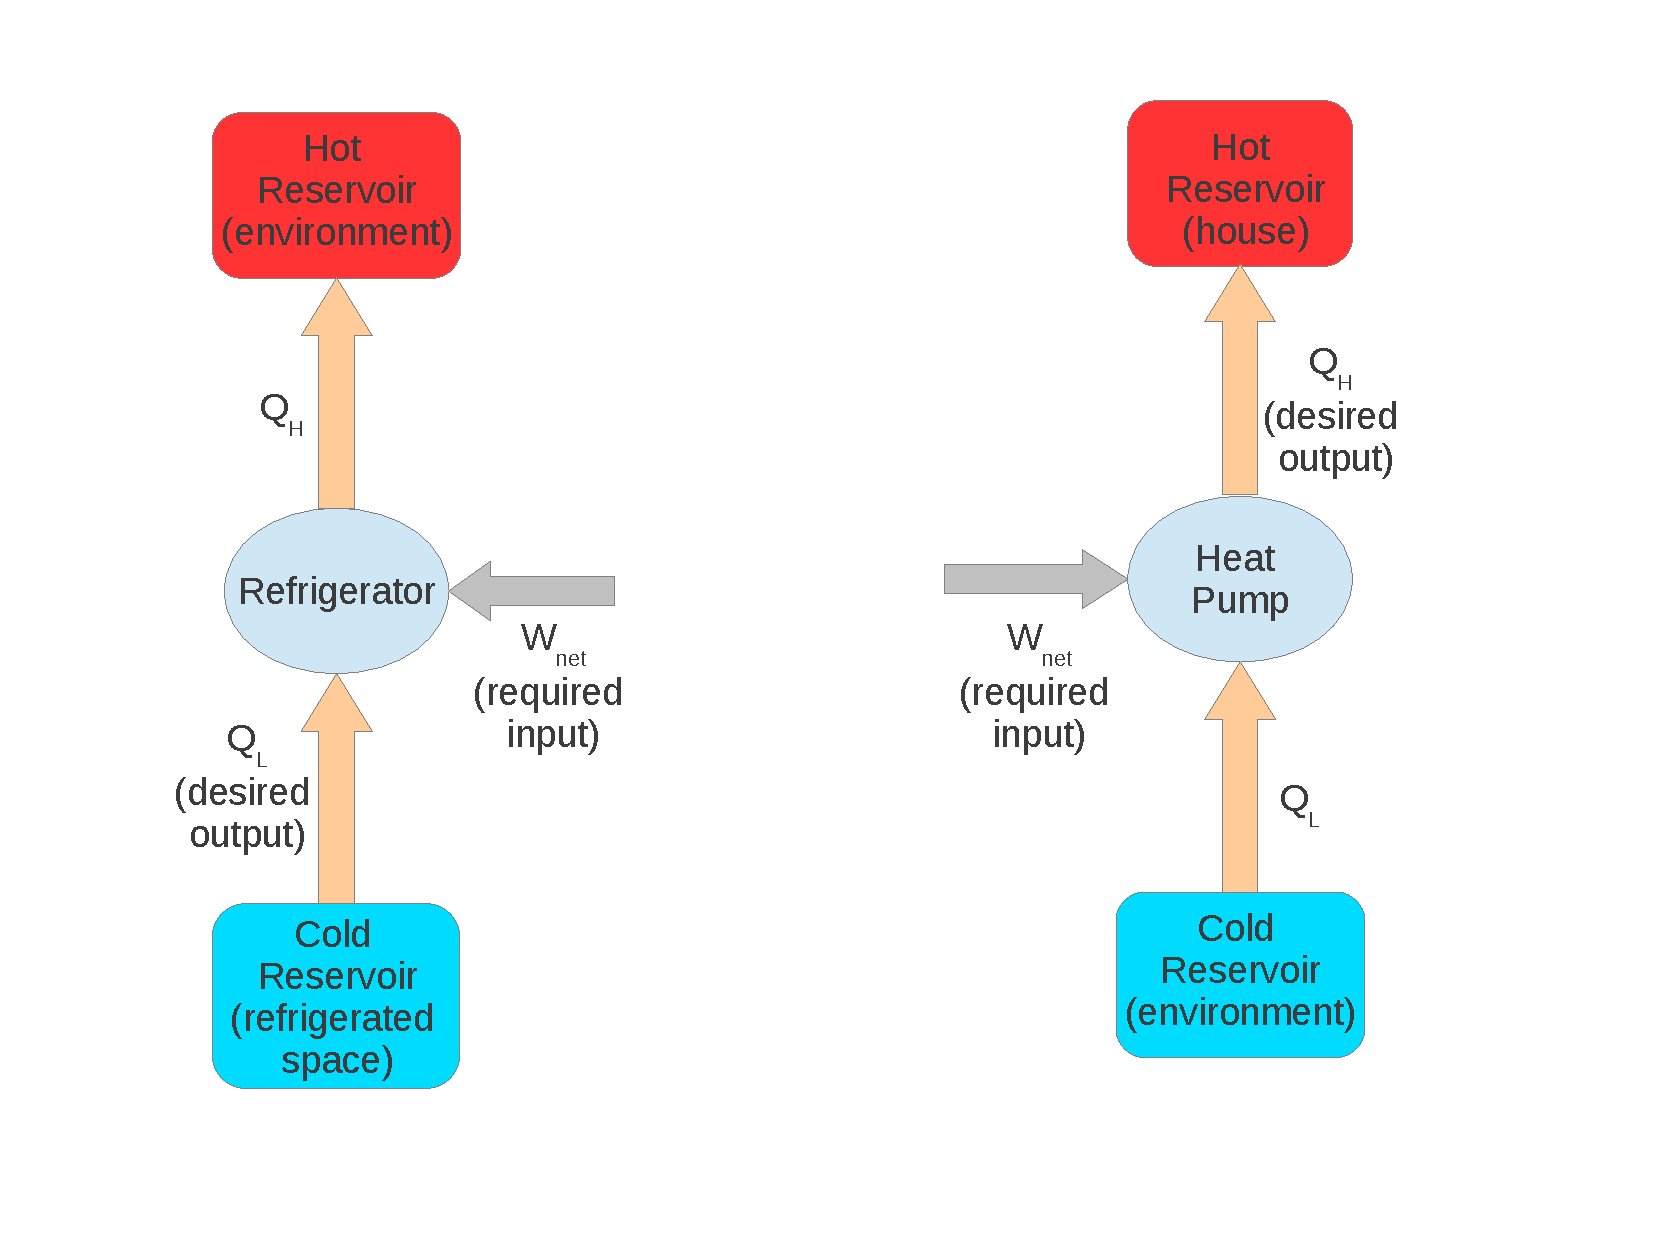
\includegraphics[width=7.5cm,clip]{./Pics/Overview_Refrig2}
     \end{center}
    \end{figure}  
   \end{column}  
  \end{columns}
\end{frame}

%%%
%%% Slide
%%%
\begin{frame}
 \frametitle{Heat Pump}
    \begin{figure}%
     \begin{center}
      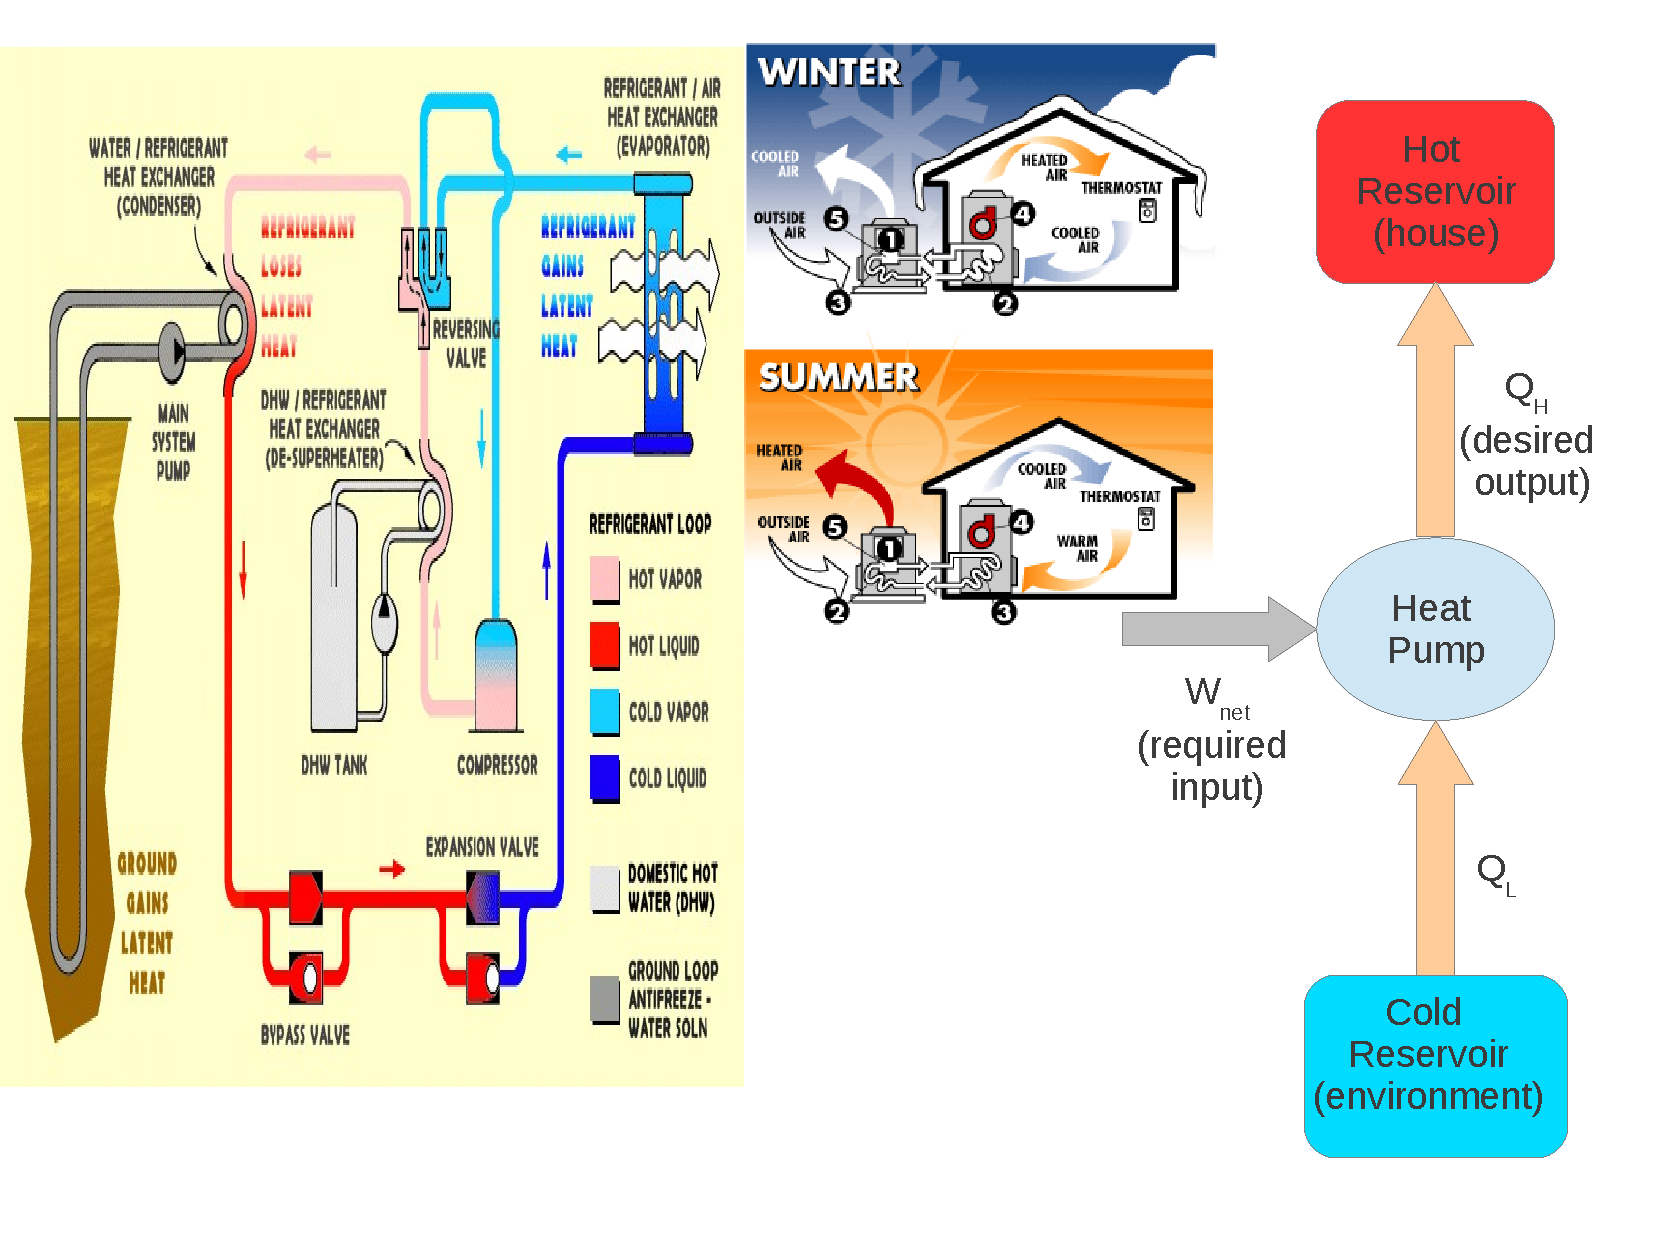
\includegraphics[width=12.cm,height=7.8cm]{./Pics/Overview_Refrig35}
     \end{center}
    \end{figure}
\end{frame}


\subsection{Reversed Carnot Cycle}
%%%
%%% Slide
%%%
\begin{frame}
 \frametitle{Objectives}
  \begin{columns}
   \begin{column}[c]{0.45\linewidth}
  \begin{enumerate}[(i)]
   \item <1-> \textcolor{blue}{Heat Pumps} are devices that are used to \textcolor{blue}{maintain} a body at a temperature larger than the surroundings;
   \item <2-> They work in a very similar way as the refrigerators we have studied, but with \textcolor{red}{a difference} in the objective;
   \item <3-> \textcolor{blue}{HPs} keep the temperature of the body above to the temperature in the surroundings whereas;
   \item <4-> The \textcolor{blue}{refrigerators} maintain the temperature below the surrounding temperature.
  \end{enumerate}
   \end{column}
   \begin{column}[c]{0.55\linewidth}
    \begin{figure}%
     \begin{center}
      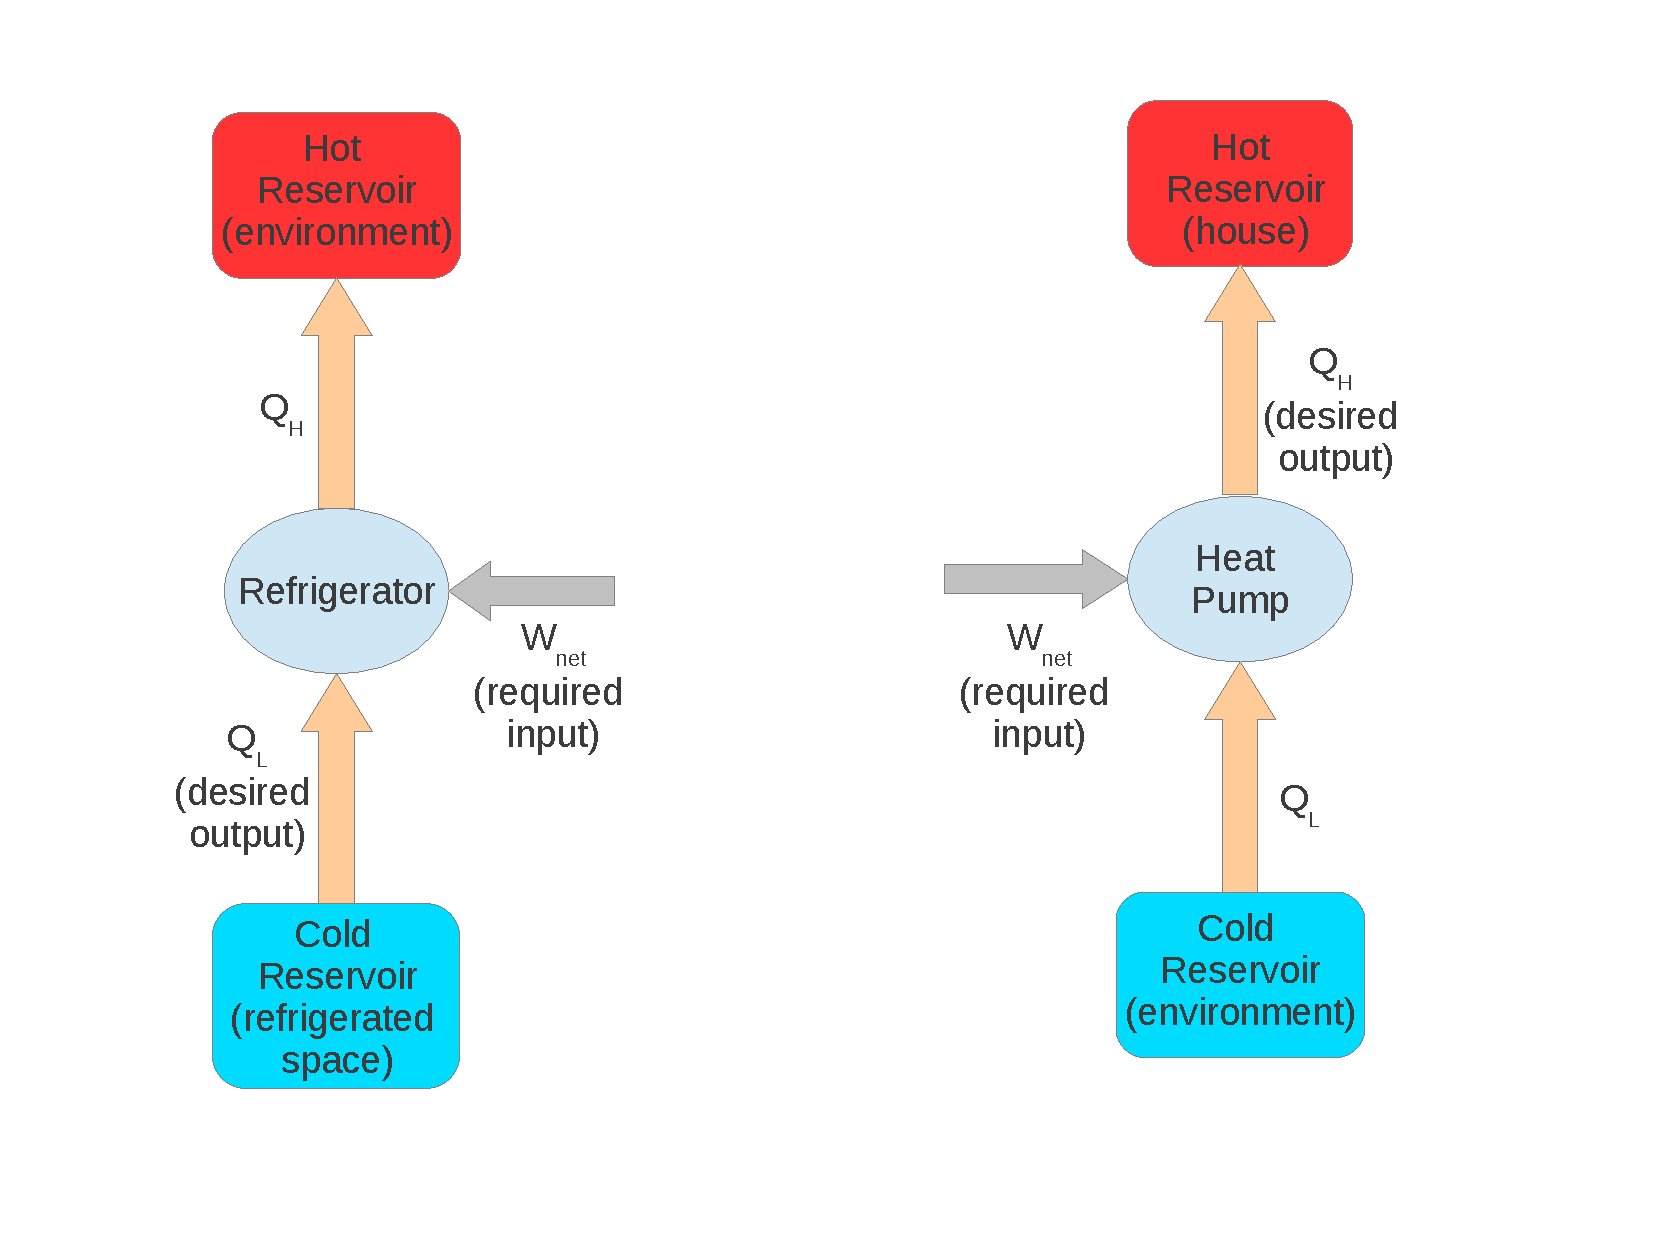
\includegraphics[width=7.5cm,clip]{./Pics/Overview_Refrig2}
     \end{center}
    \end{figure}  
   \end{column}  
  \end{columns}
\end{frame}


%%%
%%% Slide
%%%
\begin{frame}
 \frametitle{}
  \begin{columns}
   \begin{column}[c]{0.45\linewidth}
  \begin{enumerate}[(i)]
   \item <1-> \textcolor{blue}{HPs} can be based on vapour-compression cycle, absorption cycle, etc;
   \item <2-> \textcolor{blue}{Reversed Carnot cycle} is the thermodynamic cycle for \textcolor{blue}{HP};
   \item <3-> The figure in the rhs is a vapour-compression cycle representation of the heat pump;
   \item <4-> Where \textcolor{blue}{heat} is removed in the \textcolor{blue}{condenser}.
  \end{enumerate}
   \end{column}
   \begin{column}[c]{0.55\linewidth}\vspace{-1.cm}
    \begin{figure}%
     \begin{center}
      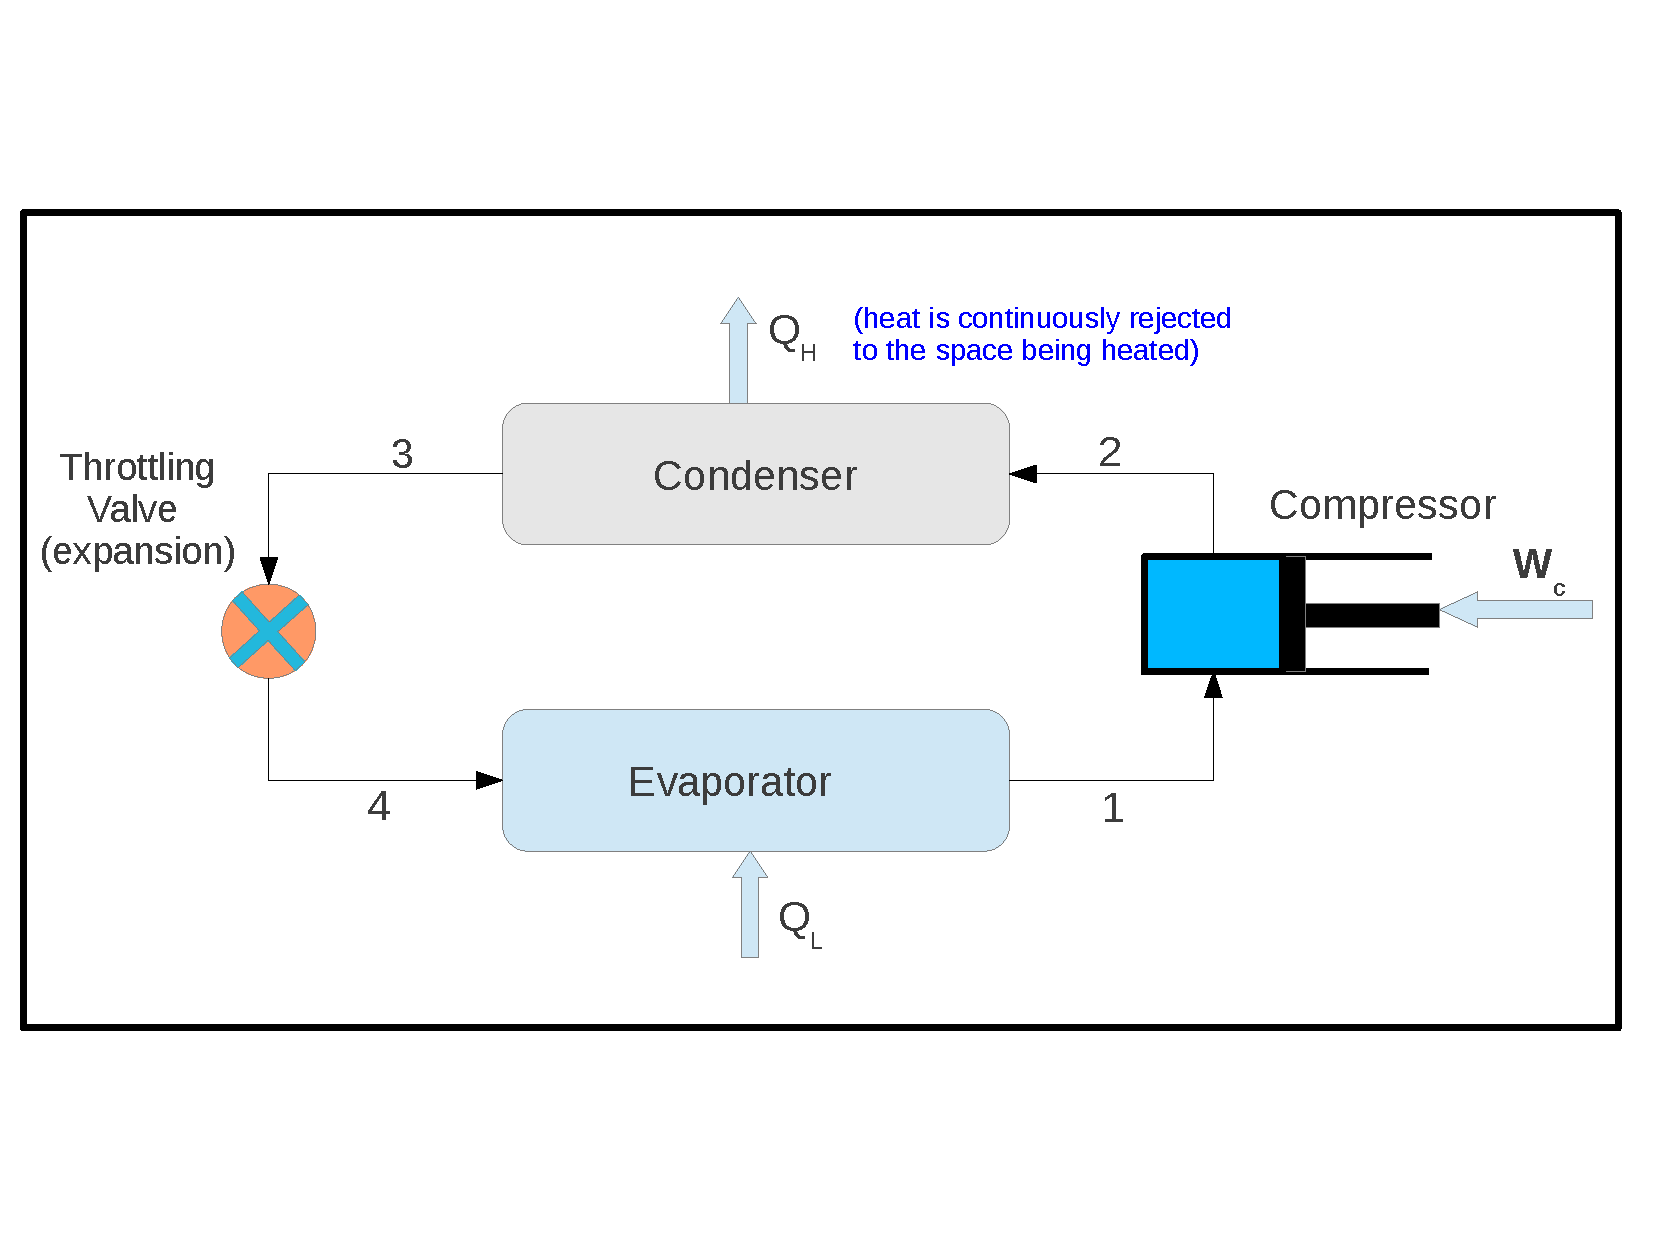
\includegraphics[width=6.5cm,clip]{./Pics/Overview_Refrig36}
     \end{center}
    \end{figure}  
   \end{column}  
  \end{columns}
\end{frame}



%%%
%%% Slide
%%%
\begin{frame}
 \frametitle{}
    \begin{figure}%
     \begin{center}
      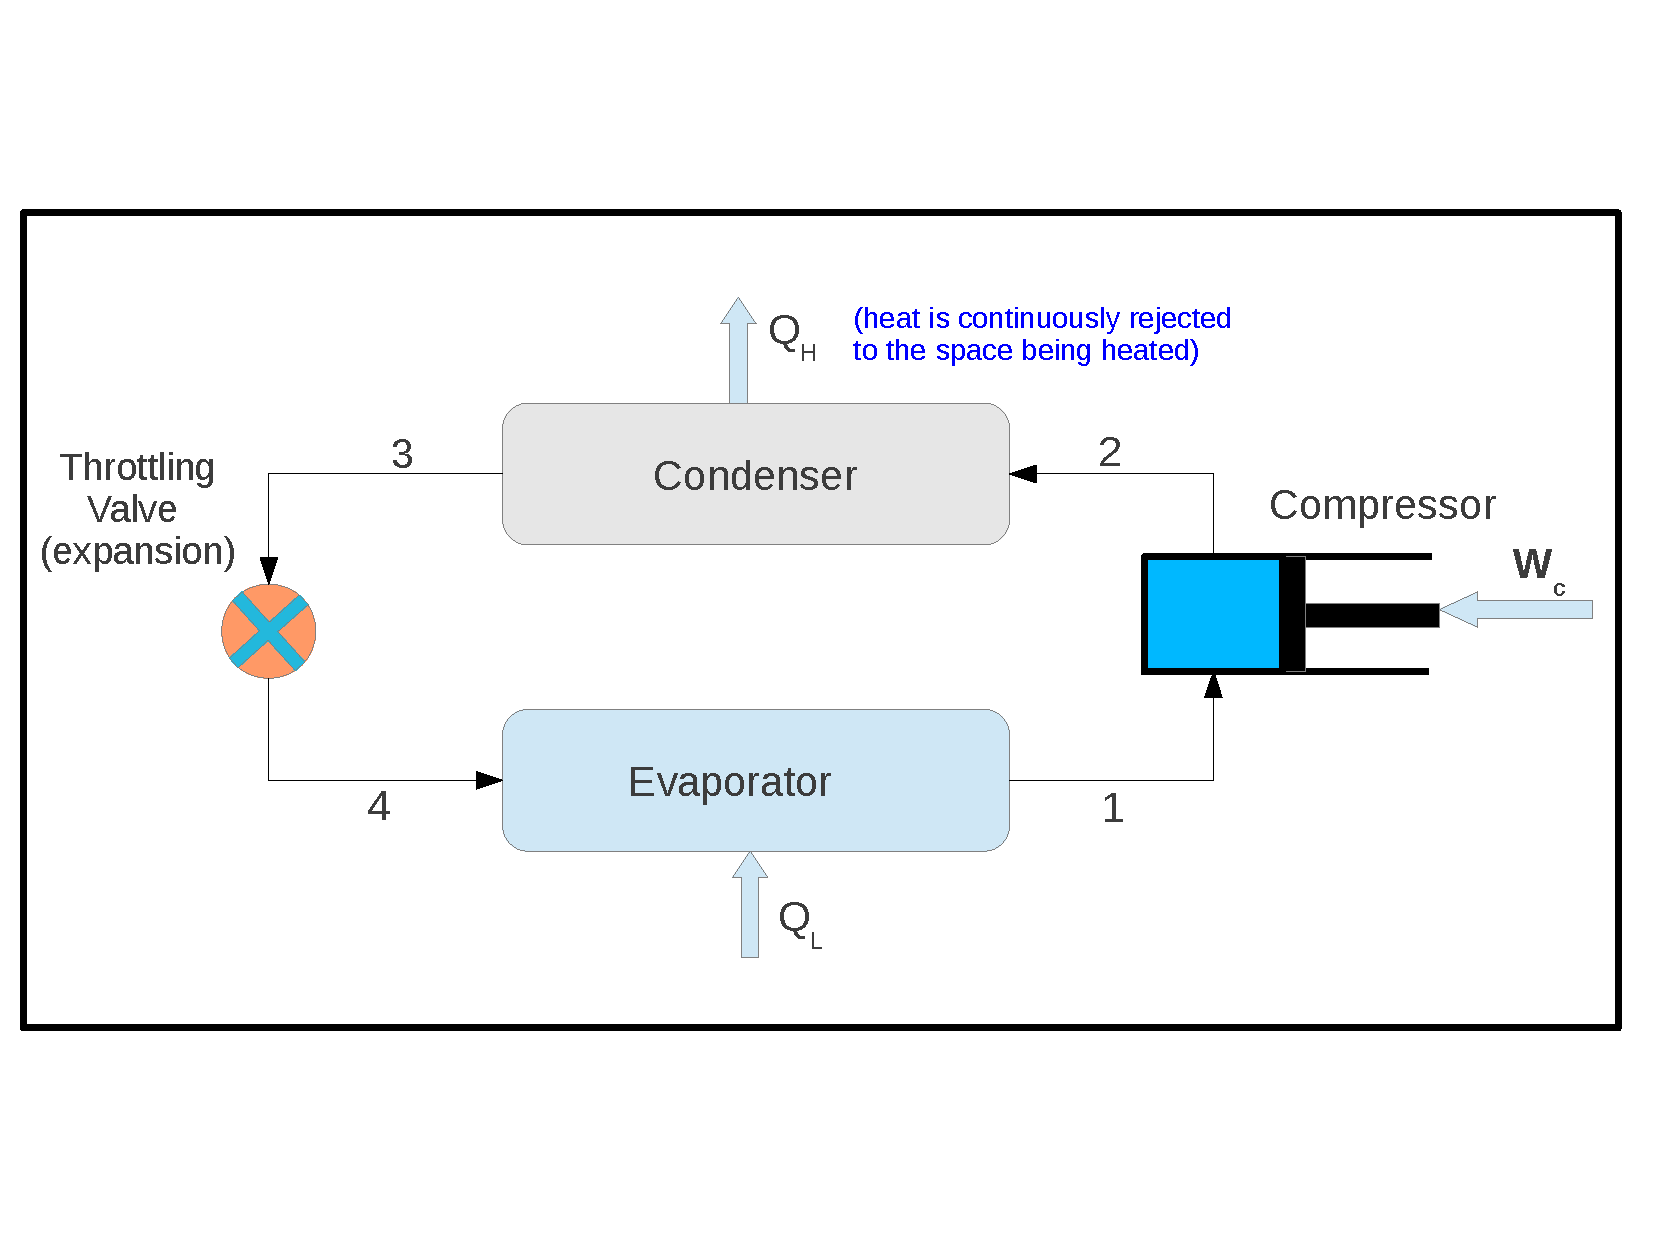
\includegraphics[width=6.5cm,clip]{./Pics/Overview_Refrig36}
     \end{center}
    \end{figure} 


  \begin{enumerate}[(i)]
   \item <1-> The \textcolor{blue}{The Coefficient of Performance} is given by
    \begin{eqnarray}
     \textcolor{blue}{\text{COP}} &=& \frc{\text{Desired Effect (heating of space)}}{\text{Net Work}} \nonumber \\
                                  &=& \frc{m\left(H_{3}-H_{2}\right)}{m\left(H_{2}-H_{1}\right)} = \textcolor{blue}{\frc{H_{3}-H_{2}}{H_{2}-H_{1}}}\nonumber
    \end{eqnarray}
   \item <2-> \textcolor{blue}{COP of Heat Pumps} usually range from 1.5 and 4.
  \end{enumerate}
\end{frame}



\section{Liquefaction Processes}
\subsection{Introduction}
%%%
%%% Slide
%%%
\begin{frame}
 \frametitle{Liquefaction: Applications}
  \begin{enumerate}[(i)]
   \item <1-> At temperature above the critical point \textcolor{blue}{$\left(T>T_{c}\right)$}, a substance can exist in the gas phase only;
   \item <2-> Liquefied gases used in industrial applications (e.g., $He$, $H_{2}$, $N_{2}$, etc) have critical temperature well-below the usual temperature found in refrigeration processes (e.g., $T_{c}^{\text{He}}=-268^{\text{o}}\text{C}$)
   \item <3-> This gasses can not exist at liquid phase at room temperature and require specific processes;
   \item <4-> Main applications are:
    \begin{enumerate}[(a)]
     \item <5-> Liquid oxygen in rockets;
     \item <6-> Liquid natural gas for ocean transportation;
     \item <7-> Liquid nitrogen for low temperature refrigeration;
     \item <8-> Liquid propane fro domestic fuel;
     \item <9-> Air is liquefied for separation (fractionation), etc;
    \end{enumerate}
   \item <10-> In a \textcolor{blue}{liquefaction process} the gas is cooled to a temperature within the \textcolor{blue}{two-phase region}.
  \end{enumerate}
\end{frame}

\subsection{Procedures for Gas Liquefaction}
%%%
%%% Slide
%%%
\begin{frame}
 \frametitle{(1) Heat exchange at constant pressure}
Heat exchange at constant pressure -- drop in the temperature field;

    \begin{figure}%
     \begin{center}
      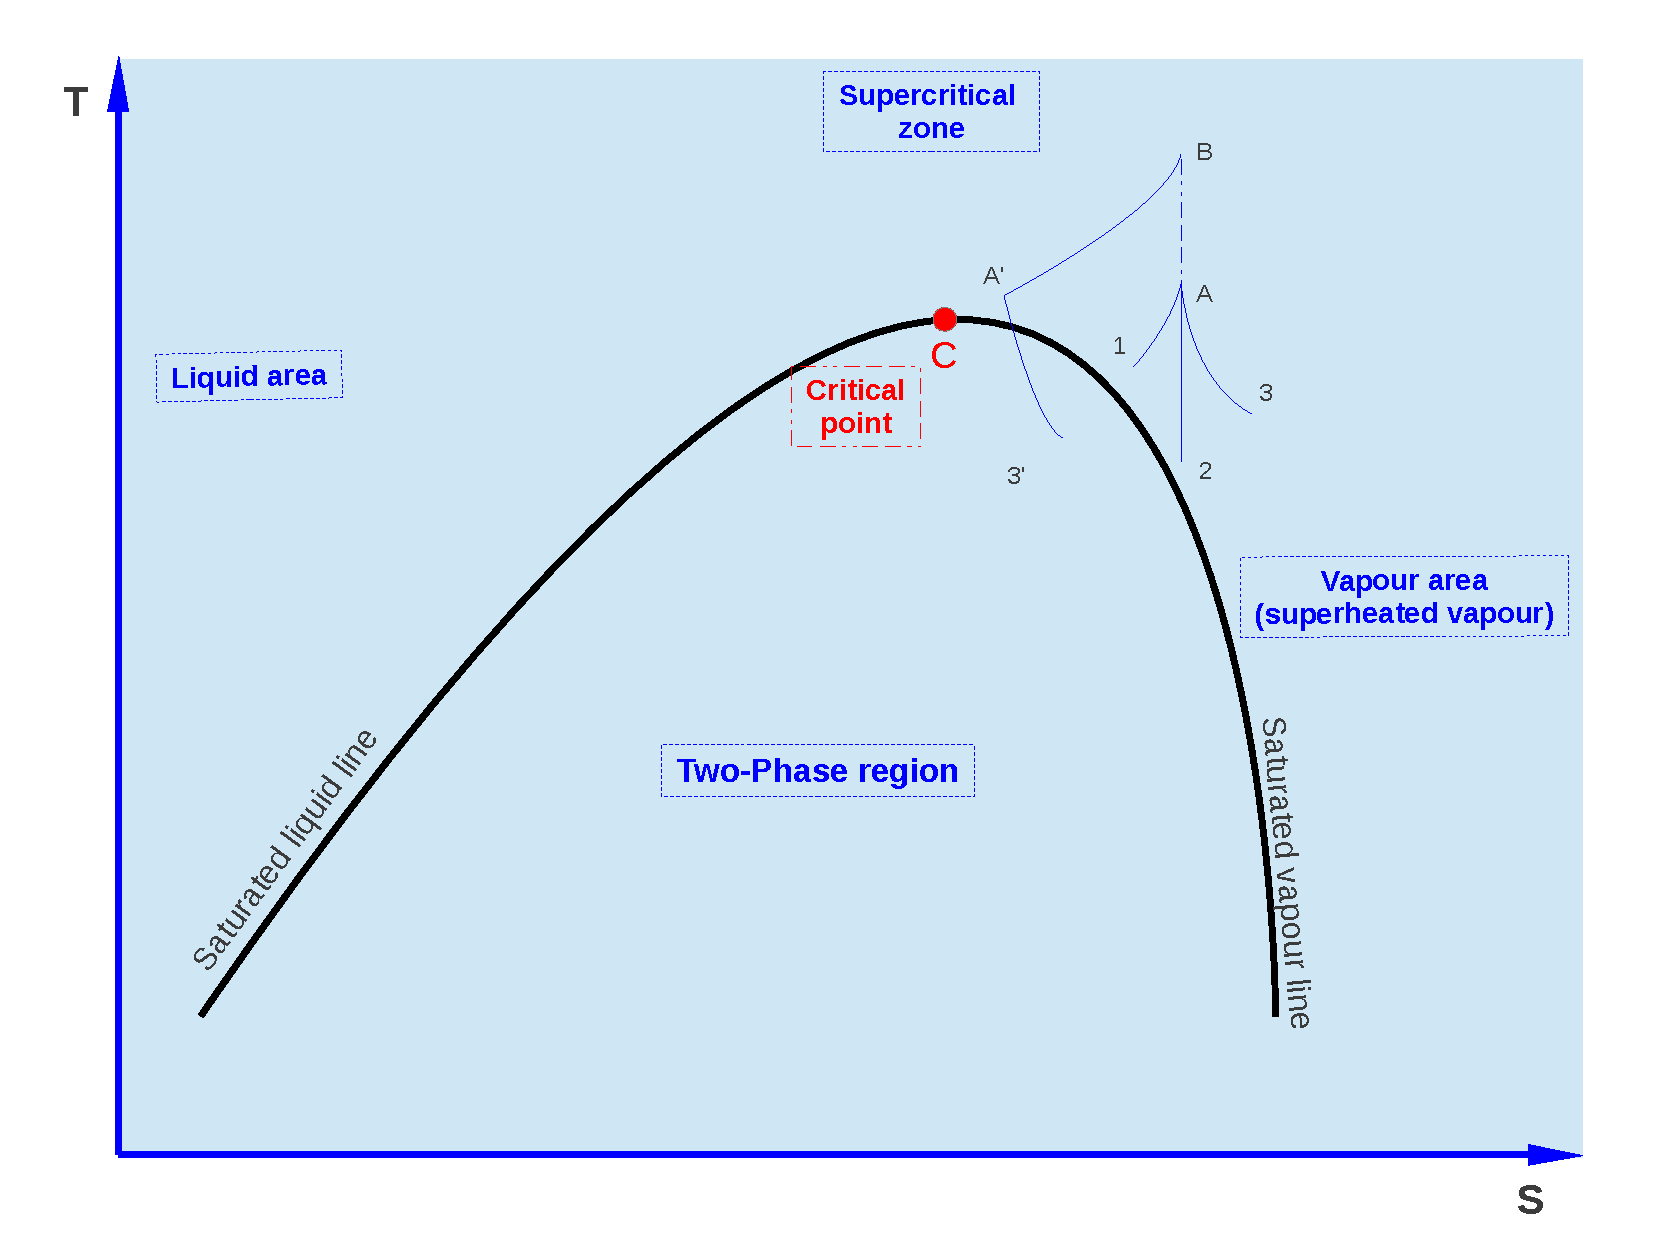
\includegraphics[width=6.5cm,clip]{./Pics/Overview_Refrig38}
     \end{center}
    \end{figure} 
\end{frame}

%%%
%%% Slide
%%%
\begin{frame}
 \frametitle{(2) Isentropic Expansion process }

    \begin{figure}%
     \begin{center}
      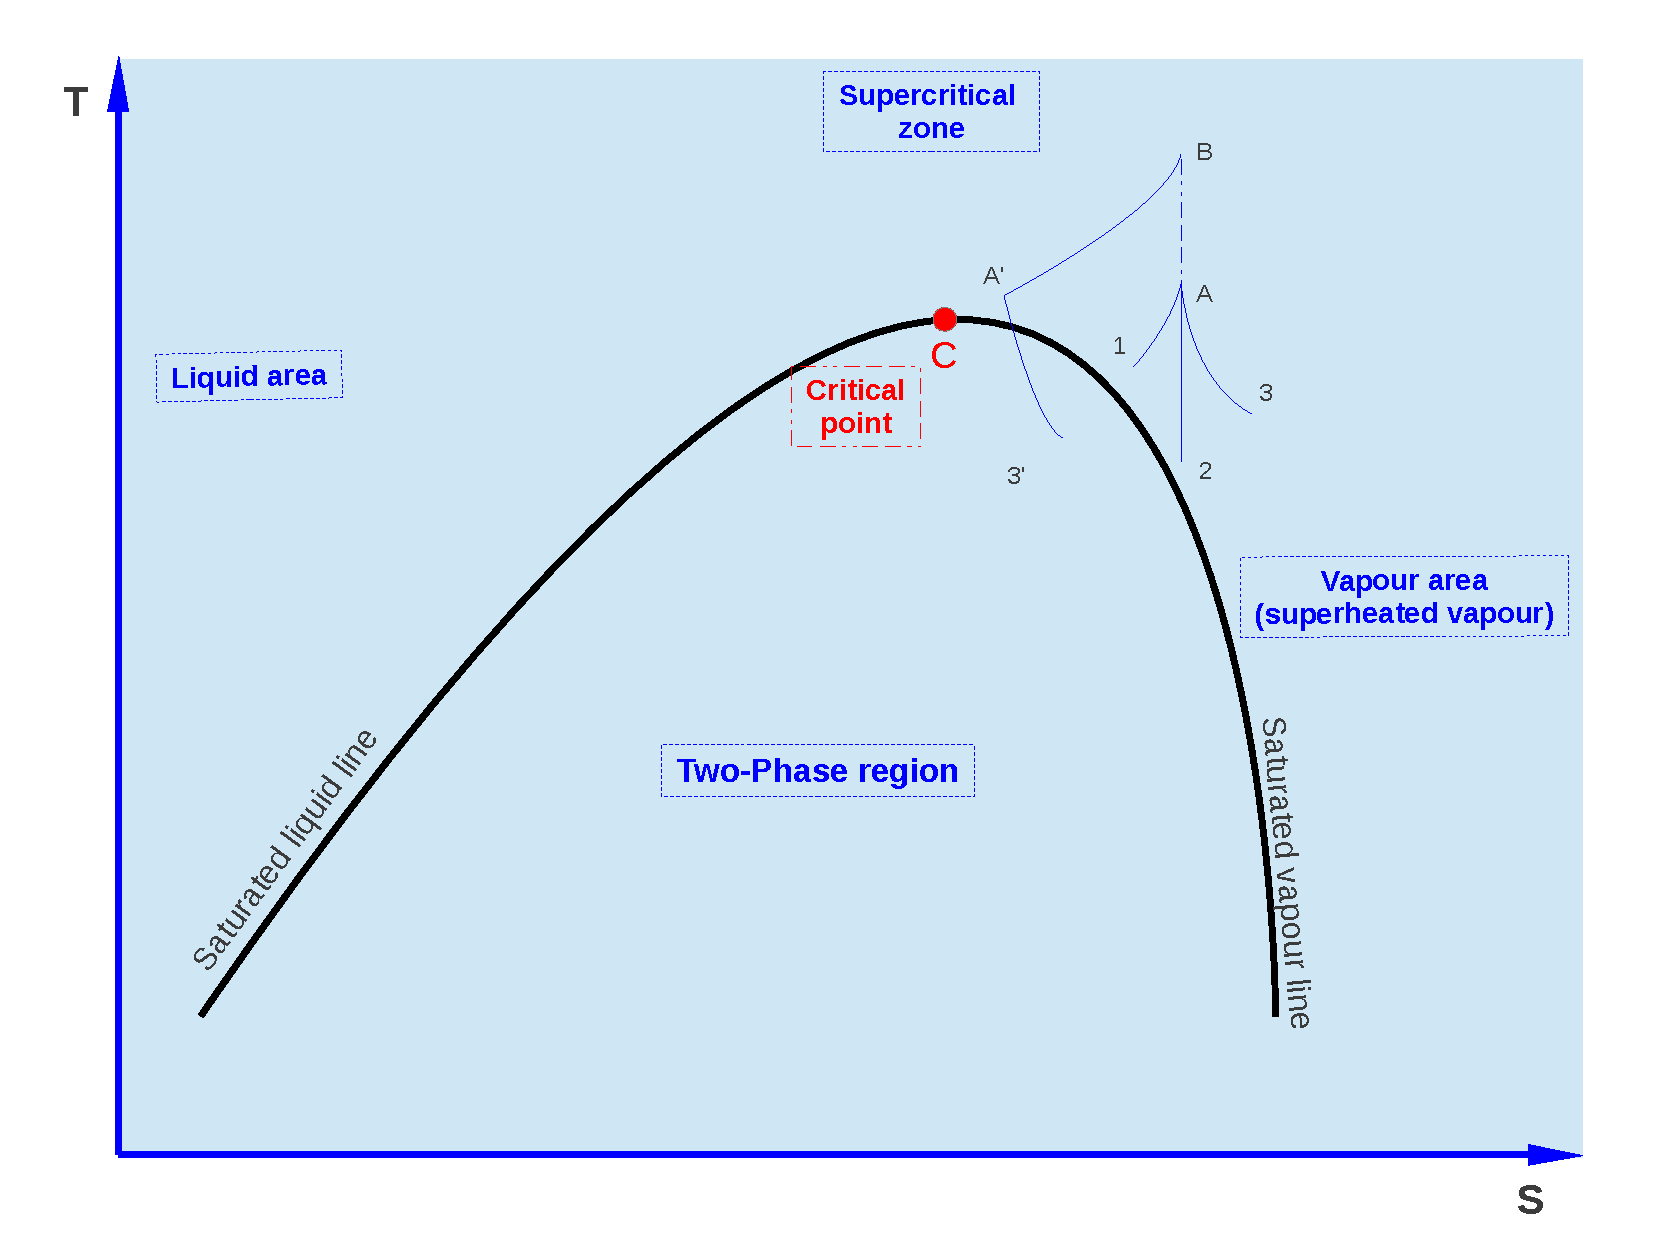
\includegraphics[width=6.5cm,clip]{./Pics/Overview_Refrig38}
     \end{center}
    \end{figure} 
\end{frame}


%%%
%%% Slide
%%%
\begin{frame}
 \frametitle{(3) Throttling process}
  \begin{columns}
   \begin{column}[c]{0.45\linewidth}
  \begin{enumerate}[(1)]
   \item <1-> It must start at high pressure and (relatively) low temperature and the isenthalpic process leads into a 2-phase region;
   \item <2-> The gas is compressed from \textcolor{blue}{A} to \textcolor{blue}{B}; 
   \item <3-> Followed by a \textcolor{blue}{constant-pressure cooling} to \textcolor{blue}{A'};
   \item <4-> Then \textcolor{blue}{isenthalpic expansion} from \textcolor{blue}{A'} to \textcolor{blue}{3'}.
  \end{enumerate}
   \end{column}
   \begin{column}[c]{0.55\linewidth}
    \begin{figure}%
     \begin{center}
      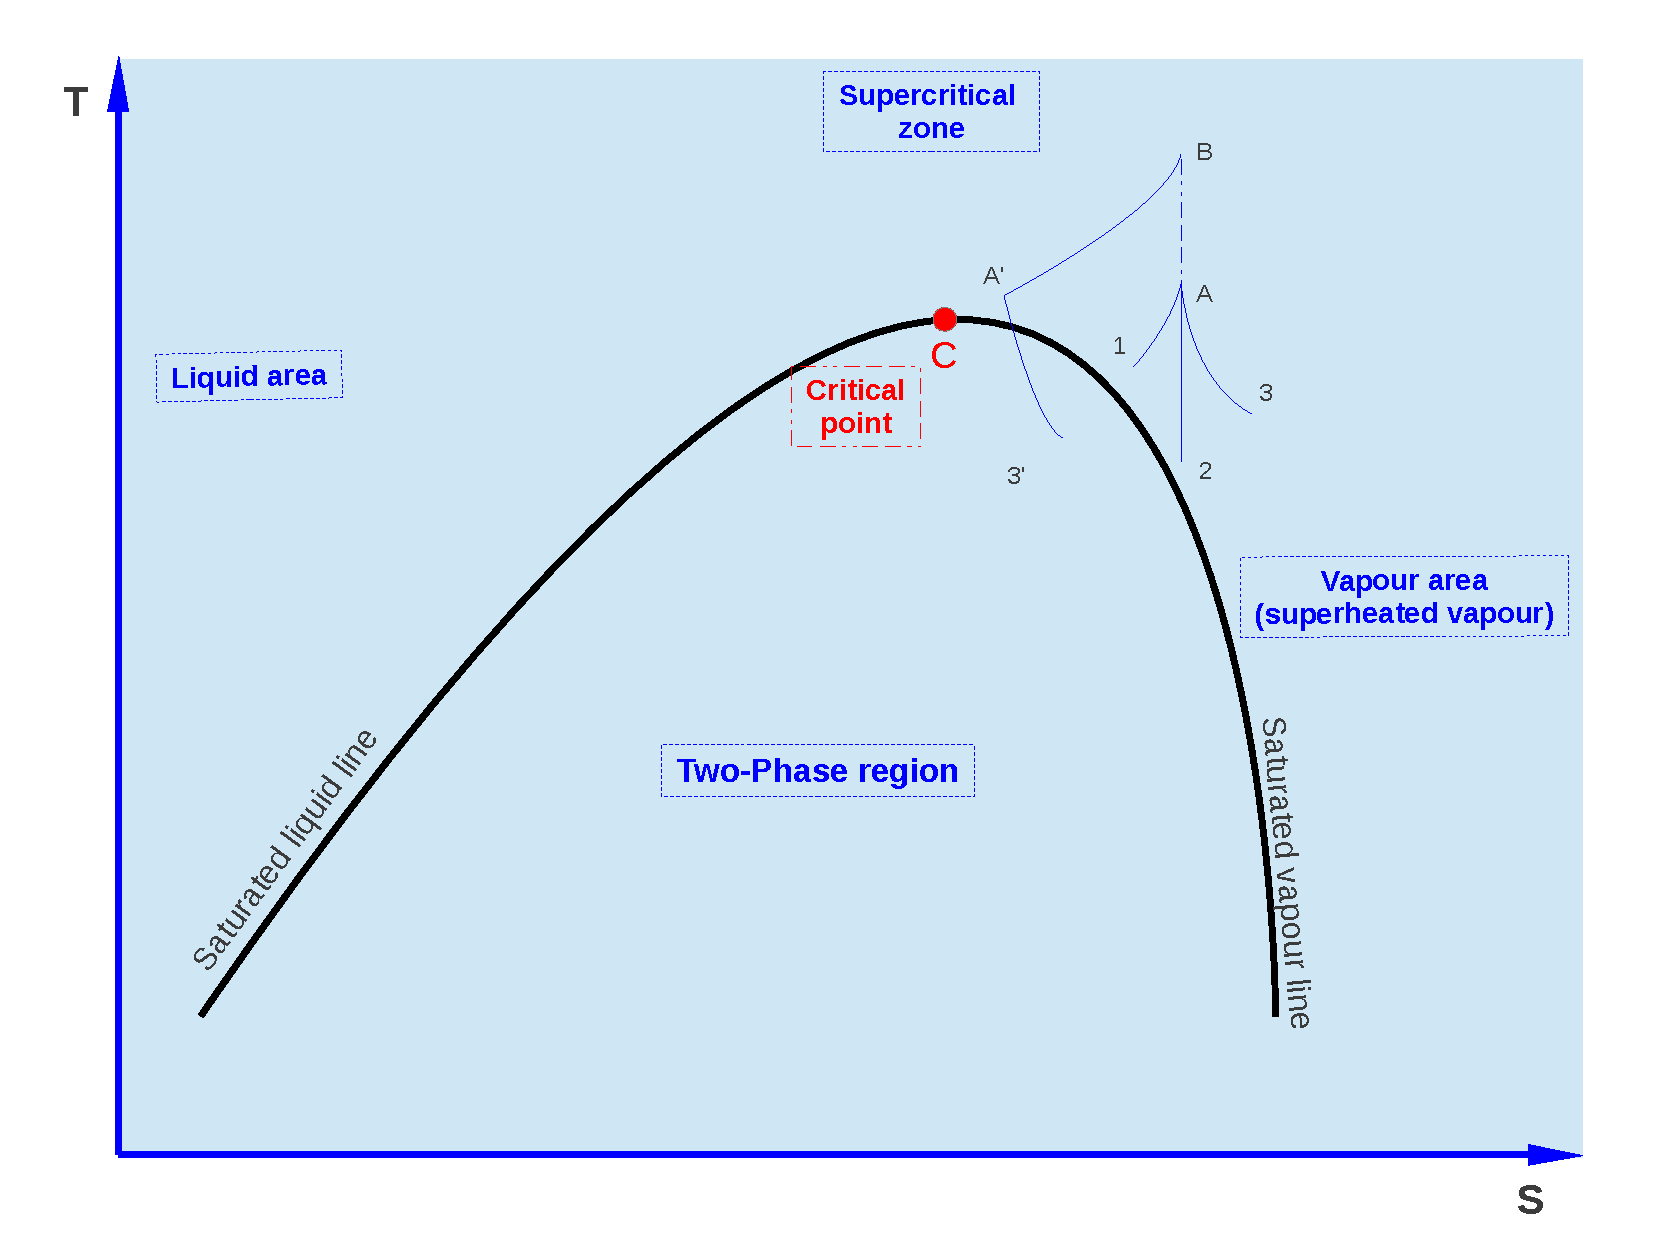
\includegraphics[width=6.5cm,clip]{./Pics/Overview_Refrig38}
     \end{center}
    \end{figure}  
   \end{column}  
  \end{columns}
\end{frame}

\subsection{Technological Applications for the Throttling Process}
%%%
%%% Slide
%%%
\begin{frame}
 \frametitle{The Linde Liquefaction Process}
  \begin{columns}
   \begin{column}[c]{0.45\linewidth}
  \begin{enumerate}[(1)]
   \item <1-> After the compression, the gas is pre-cooled to room temperature (or lower via ordinary refrigeration) -- \textcolor{blue}{3-5};
   \item <2-> The lower the temperature entering the throttling valve the larger the fraction of the gas that can be liquefied; 
   \item <3-> A fraction of the liquefied gas is removed and the gas phase is returned into the cycle for further compression and extraction.
  \end{enumerate}
   \end{column}
   \begin{column}[c]{0.55\linewidth}
    \begin{figure}%
     \begin{center}
      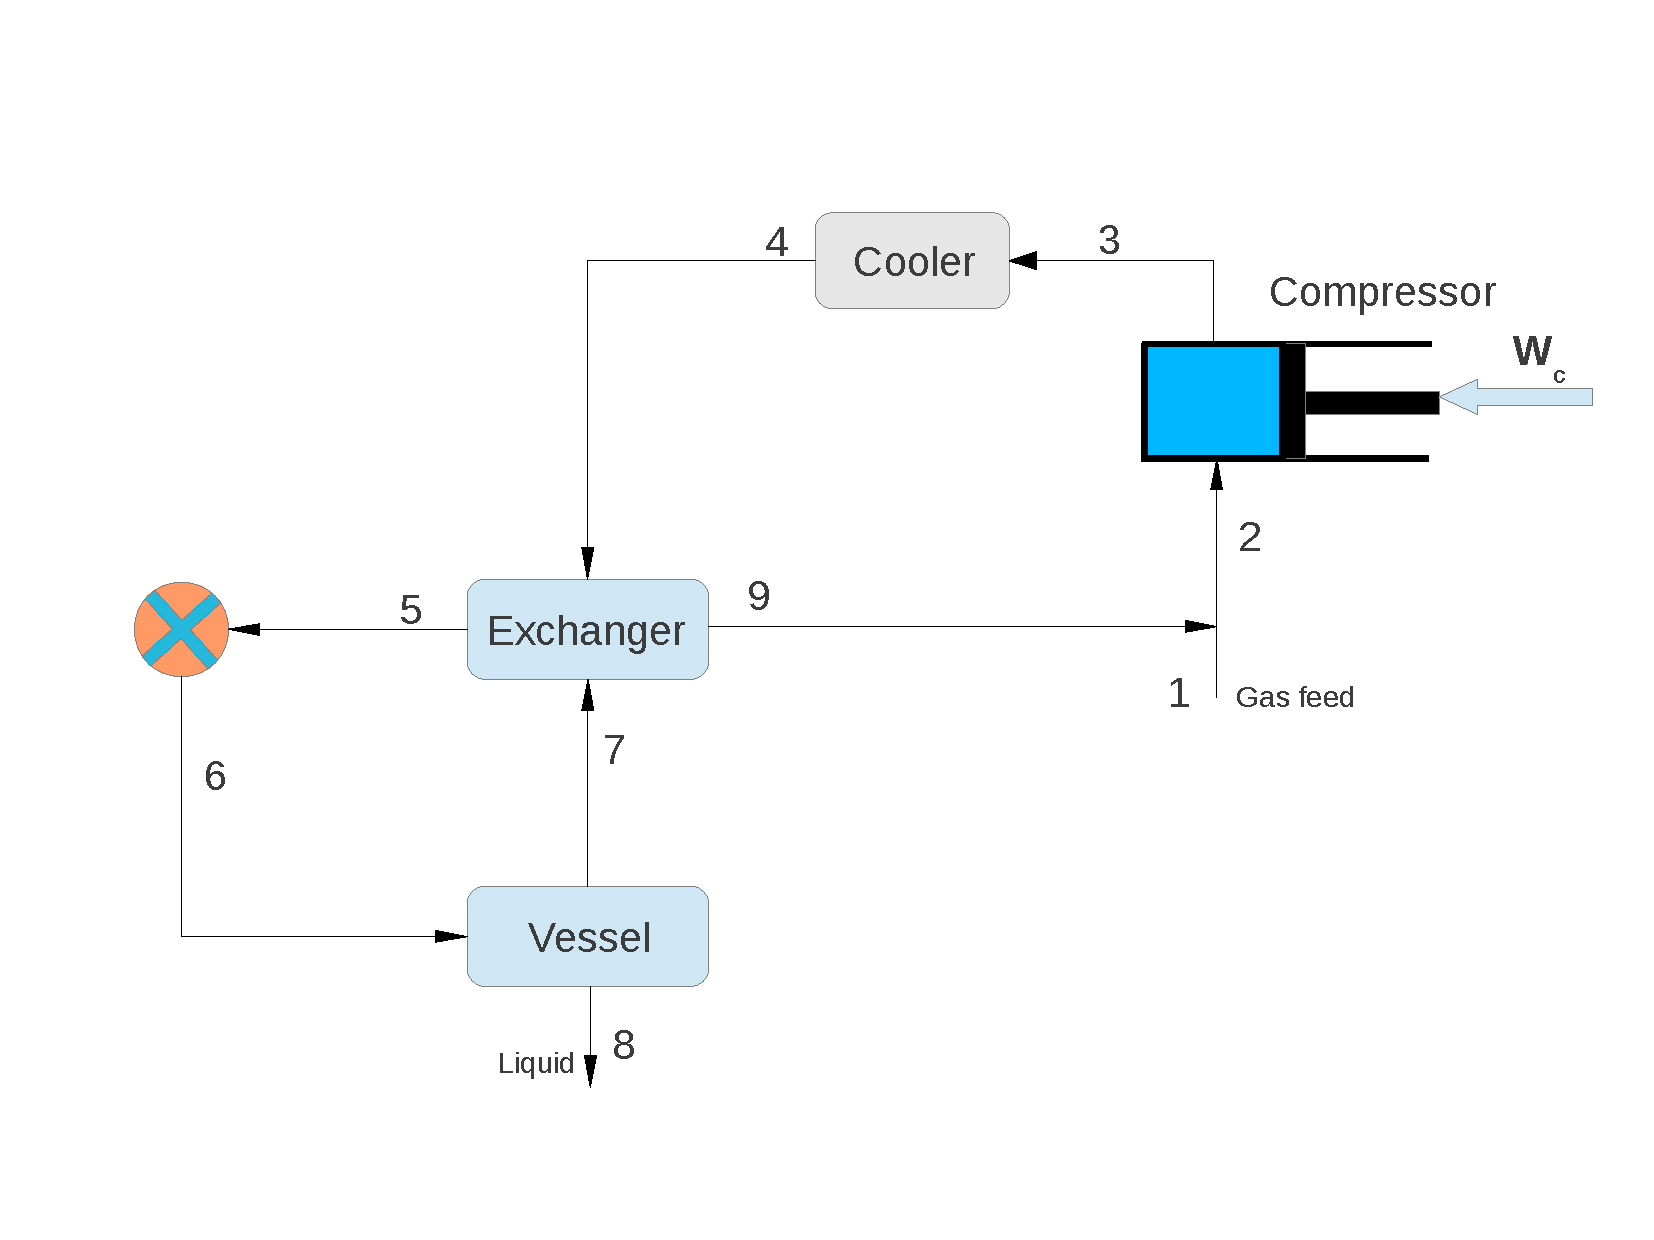
\includegraphics[width=6.5cm,clip]{./Pics/Overview_Refrig39}
     \end{center}
    \end{figure}  
   \end{column}  
  \end{columns}
\end{frame}

%%%
%%% Slide
%%%
\begin{frame}
 \frametitle{The Claude Liquefaction Process}
  \begin{columns}
   \begin{column}[c]{0.45\linewidth}
  \begin{enumerate}[(1)]
   \item <1-> Based upon the idea of replacing the throttle valve by an expander to improve the efficiency of the process;
   \item <2-> Gas at \textcolor{blue}{intermediate temperature} is obtained from the \textcolor{blue}{heat exchanger system}; 
   \item <3-> The gas \textcolor{red}{(11)} is driven to the \textcolor{blue}{expander} producing either \textcolor{blue}{saturated} or \textcolor{blue}{slightly superheated} vapour;
   \item <4-> Another fraction of the gas \textcolor{red}{(5)} from the \textcolor{blue}{exchanger} is further cooled and throttled \textcolor{red}{(7)} to produce liquefaction liquid (similar to the Linde process).
  \end{enumerate}
   \end{column}
   \begin{column}[c]{0.55\linewidth}
    \begin{figure}%
     \begin{center}
      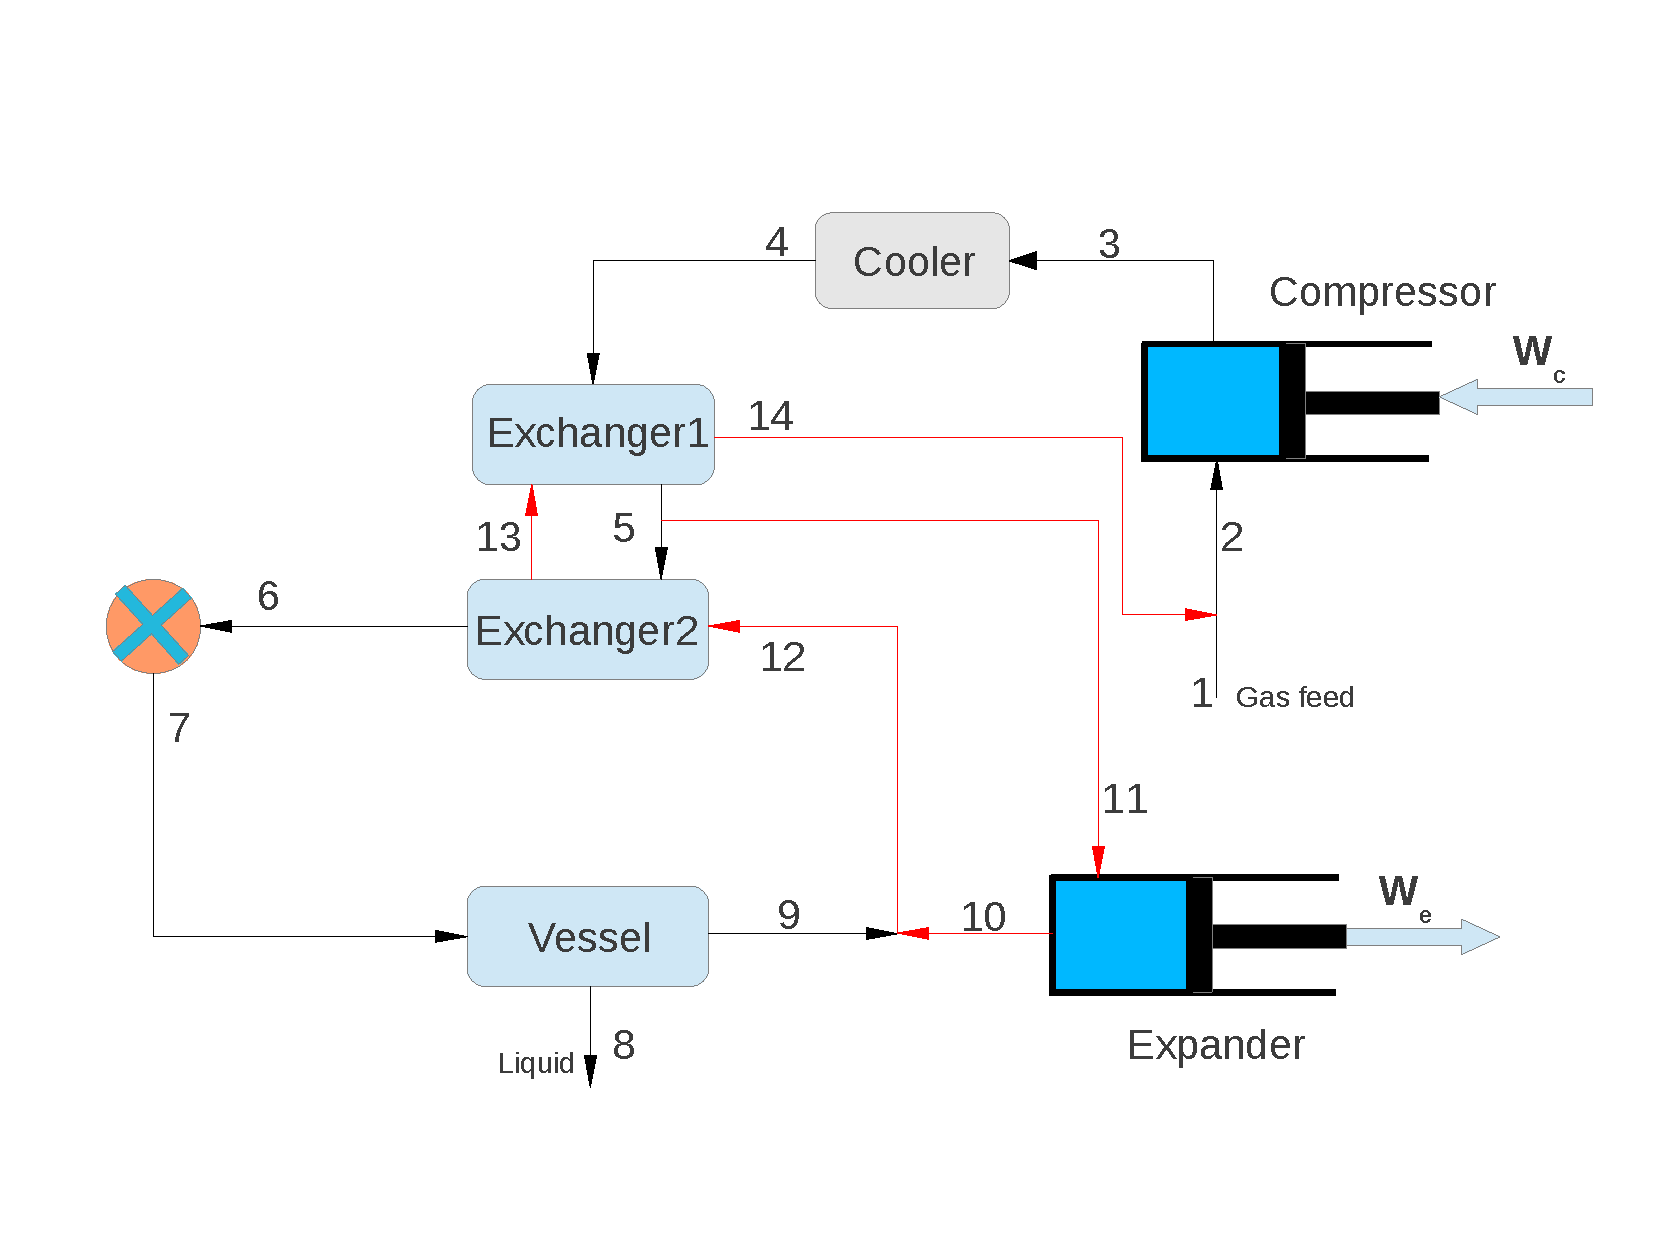
\includegraphics[width=6.5cm,clip]{./Pics/Overview_Refrig40}
     \end{center}
    \end{figure}  
   \end{column}  
  \end{columns}
\end{frame}

%%%
%%% Slide
%%%
\begin{frame}
 \frametitle{The Claude Liquefaction Process}
  \begin{columns}
   \begin{column}[c]{0.45\linewidth}
  \begin{enumerate}[(1)]
   \item <1-> The non-liquefied fraction \textcolor{red}{(9)} -- \textcolor{blue}{saturated vapour}, is mixed with the flow from the \textcolor{blue}{expander} exhaust and returns for \textcolor{blue}{recycle};
   \item <2-> As we can see, The \textcolor{blue}{Linde} process is a {\bf special (or limiting)} case of the the \textcolor{blue}{Claude} process when the high-pressure gas stream {\bf is not sent} to the expander.
  \end{enumerate}
   \end{column}
   \begin{column}[c]{0.55\linewidth}
    \begin{figure}%
     \begin{center}
      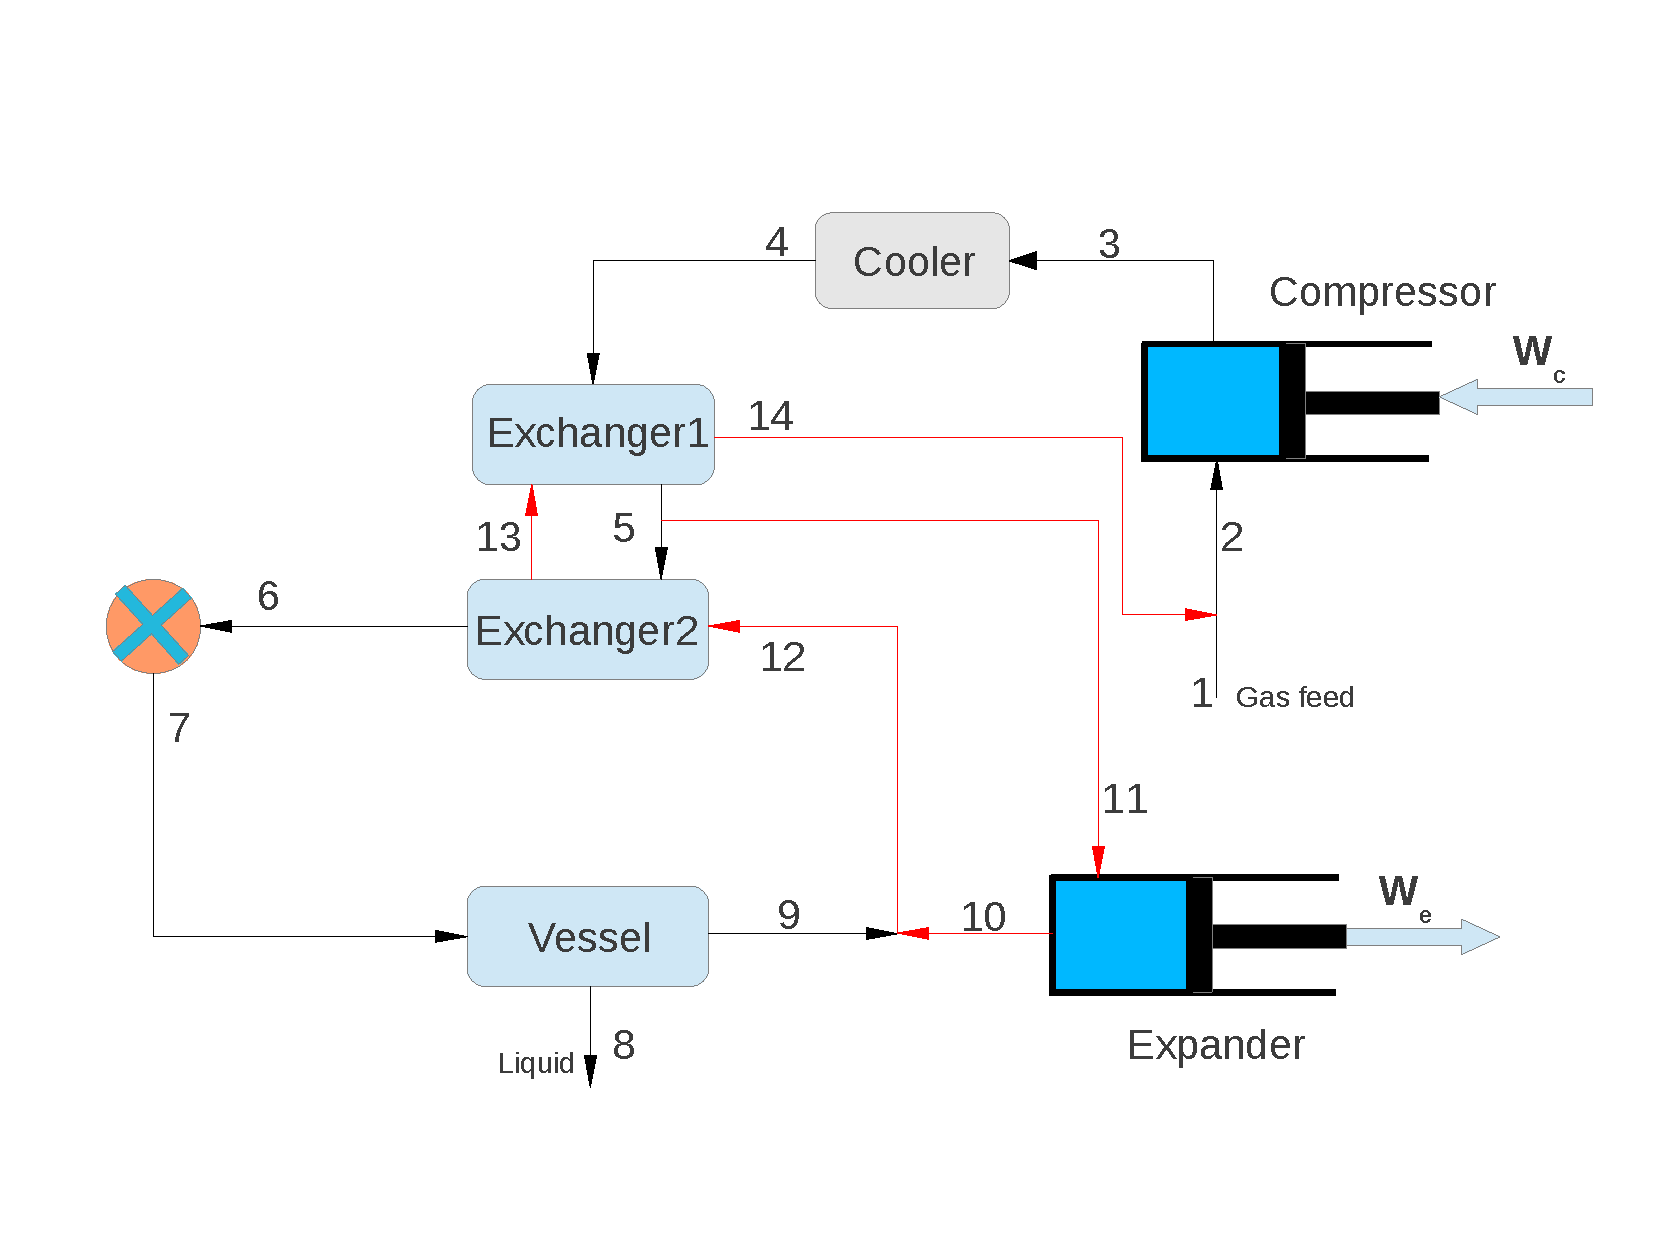
\includegraphics[width=6.5cm,clip]{./Pics/Overview_Refrig40}
     \end{center}
    \end{figure}  
   \end{column}  
  \end{columns}
\end{frame}


\section{Summary}

%%%
%%% Slides
%%%
\begin{frame}
 \frametitle{Summary}
  After this Module you should:
 \begin{enumerate}[(a)]
  \item <1-> Identify elements of the gas and vapour-compressed refrigeration systems and liquefaction processes;
  \item <2-> Link the thermo-fluid dynamics learnt in Module 3 with the use of expansion valves in Module 4;
  \item <3-> Be able to sketch $PH$ and $TS$ diagrams and perform a thermal analysis of the cycles;
  \item <4-> Identify refrigerant fluids and be able to select a fluid according to the design specification.
 \end{enumerate}
\end{frame}




\end{document}
